\documentclass{article}
\usepackage{asymptote}
\usepackage{caption}
\newcommand{\HRule}{\rule{\linewidth}{0.5mm}}

\begin{document}

\begin{titlepage}
\begin{center}
\textsc{\LARGE Team2 Inc.}\\[1.5cm]

% title
\HRule \\[1.4cm]
{ \huge \bfseries Ushahidi GeoRole Project Outline}\\[0.4cm]

\HRule \\[1.5cm]

%Author Data
\begin{minipage}{0.4\textwidth}
\begin{flushleft}
Michael Hnatiw
\end{flushleft}
\end{minipage}
\begin{minipage}{0.4\textwidth}
\begin{center}
Stephen Lind
\end{center}
\end{minipage}
\begin{minipage}{0.4\textwidth}
\begin{flushright}
Taylor Parrish
\end{flushright}
\end{minipage}

%bottom of page
\vfill
{\large \today}
\end{center}
\end{titlepage}

\section{Problem}
\subsection{Metaphor}
Using MSPaint and Google Maps as user restriction tools.
\subsection{Problem Explained}
Ushahidi currently has no way to restrict user roles based on geographic location. There are a few issues with this, namely lack of local expertise and credibility. Administrators would be well served with a feature that would allow them to select a geographic region under which their reports will be allowed to operate.

\section{Requirements}
\subsection{Mock Up}
\begin{itemize}
\item The ideal solution is to use a graphical tool to select the region. Ushahidi currently supports some form of polygon selection, however our team will need to investigate the possibility of incorporating this pre-existing code into this addition. This feature would resemble the following figure.
\begin{minipage}{\linewidth}
  \centering
  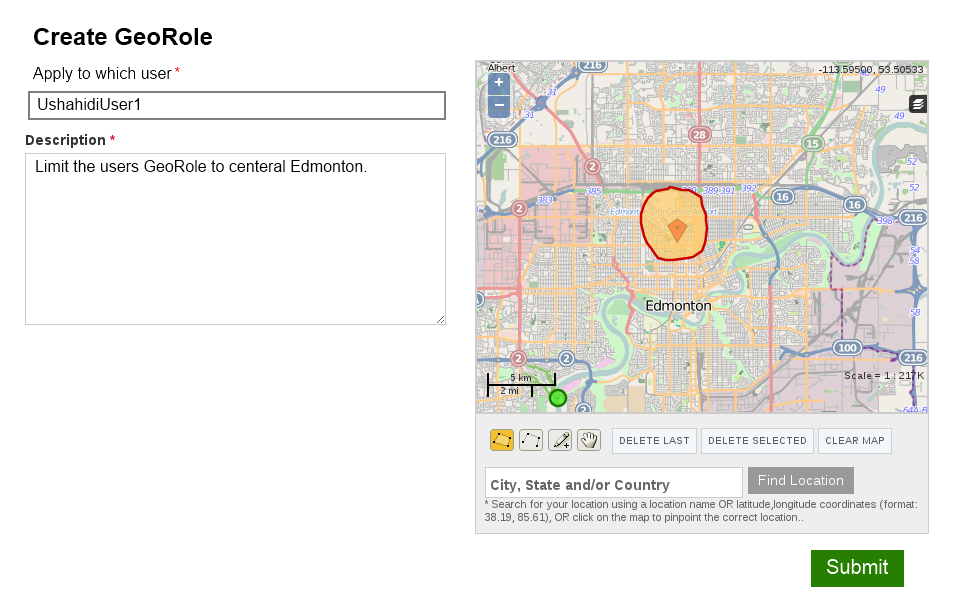
\includegraphics[width=100mm]{mockupMap.png}
  \captionof{figure}{Map based region selection.}
\end{minipage}
\item The more simplistic approach is to define a region based on text input. This may prove to be the more ideal solution if the pre-existing map based polygon hooks prove difficult to implement in our addition.
\end{itemize}
\begin{minipage}{\linewidth}
  \centering
  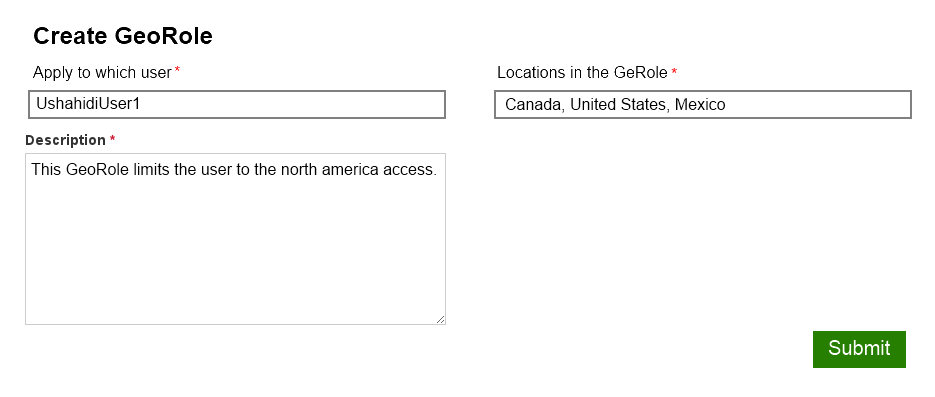
\includegraphics[width=100mm]{mockupNomap.png}
  \captionof{figure}{Text based region selection}
\end{minipage}
\subsection{User Stories}
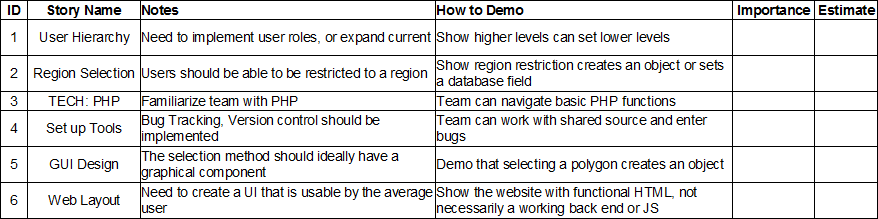
\includegraphics[width=100mm]{ProjectBacklogImage.png}
\subsection{Must Haves}
-User hierarchy of geographic restriction.
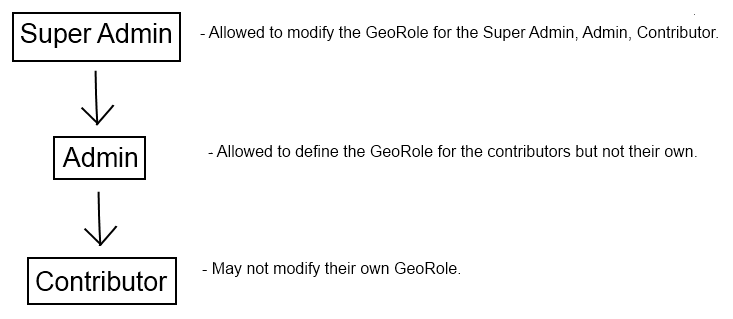
\includegraphics[width=100mm]{permissions.png}
-Some representation to the user of area of restriction or control.

\section{Time Line}
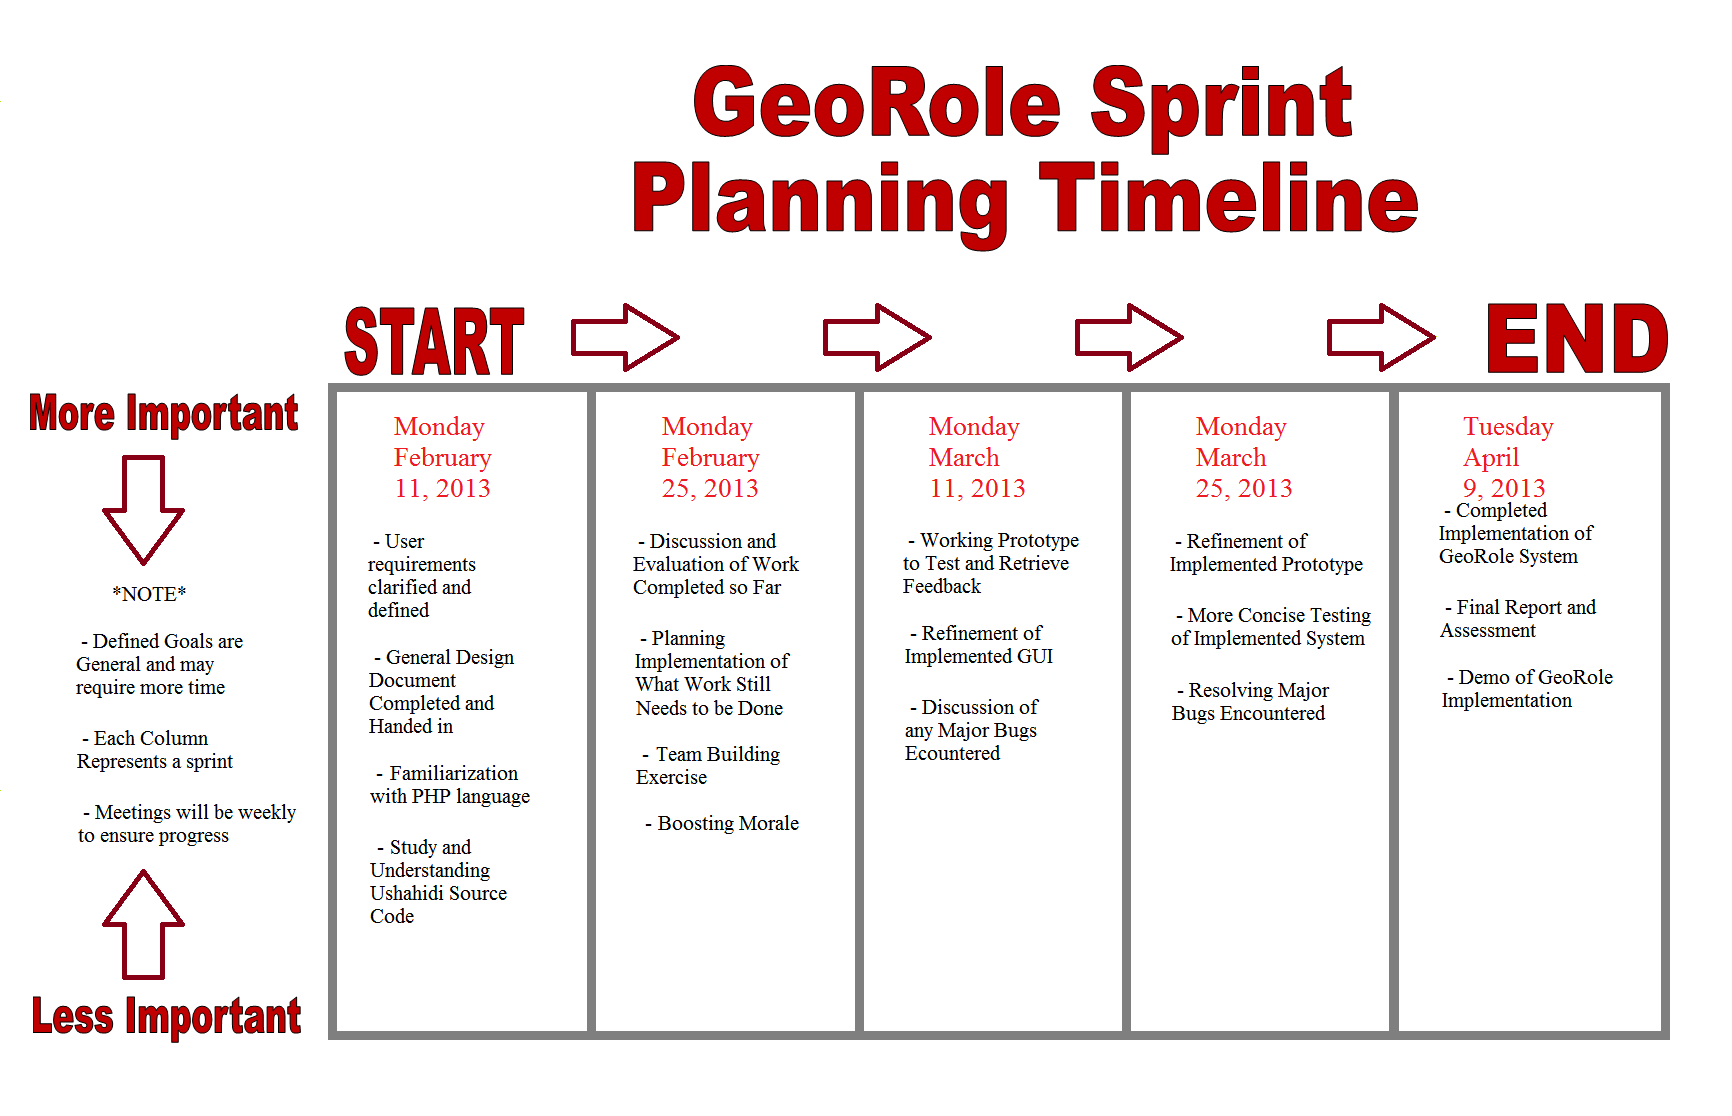
\includegraphics[width=100mm]{UshahidiTimeline.png}

\section{Approach}
As Ushahidi's web framework runs on Kohana, this will naturally be an extension of the Model-View-Controller. At a more specific level, we will be using a modified scrum development scheme. As we are a small team we will not have a traditional Product Owner or Scrum Master. We as a team will decide the weighting and importance of user stories and incorporate them into the sprints themselves.

\section{Obstacles}
\subsection{Unknowns}
Ushahidi's code base for GUI geographic region selection is obscure and difficult to locate. The actual object behind this functionality is currently our biggest unknown. Until there is further communication with Ushahidi developers we are at a loss for GUI development. This could turn a risk, or the option as shown in the alternative mock up is to us a text based selection.
\subsection{Risks}
-Time frame. We have 5 sprints comprising 9 weeks. Our team is involved with other tasks so we expect our focus factor to be low.
-Business risk. As we lack a project owner, the task outline is vague and our deliverable may be not as expected.
-Technological risk, our team is new to PHP and Kohana. The upside to this is as our team is brought up to speed, our focus factor should increase.
-Feature creep. As there is no project owner, our team's ambition could add to the project backlog unnecesarily.


Project Razor created with la\TeX~.
\end{document}
